\subsection{Interpretability is Consistent across Dictionary Sizes}

We find that larger interpretability scores of our feature dictionaries are not limited to overcomplete dictionaries (where the ratio, $R$, of dictionary features to model dimensions is $>1$), but occurs even in dictionaries that are smaller than the underlying basis, as shown in Figure \ref{fig:dictionary_size_comparison}. These small dictionaries are able to reconstruct the activation vectors less accurately, so with each feature being similarly interpretable, the larger dictionaries will be able to explain more of the overall variance.

\begin{figure}
    \centering
    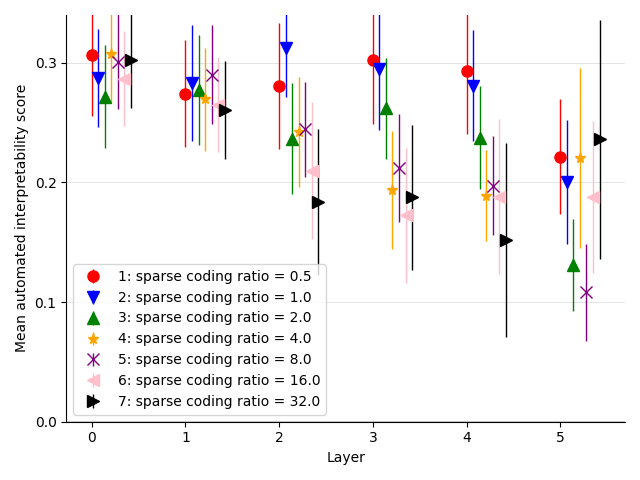
\includegraphics[width=.8\textwidth]
    {images/interp_across_ratio.png}
    \caption{Comparison of average interpretability scores across dictionary sizes. All dictionaries were trained on 20M activation vectors obtained by running Pythia-70M over the Pile with $\alpha=.00086$.}
    \label{fig:dictionary_size_comparison}
\end{figure}


\subsection{High Interpretability Scores Are Not an Artefact of Top Scoring}

A possible concern is that the autointerpretability method described in Section \ref{section:autointerp} combines top activating fragments (which are usually large) with random activations (which are usually small), making it relatively easy to identify activations. Following the lead of \citet{bills2023language}, we control for this by recomputing the autointerpretation scores by modifying Step 3 using only randomly selected fragments. With large sample sizes, using random fragments should be the true test of our ability to interpret a potential feature. However, the features we are considering are heavy-tailed, so with limited sample sizes, we should expect random samples to underestimate the true correlation.

In Figure \ref{fig:residual_random_activations} we show autointerpretability scores for fragments using only random fragments. Matching \citet{bills2023language}, we find that random-only scores are significantly smaller than top-and-random scores, but also that our learned features still consistently outperform the baselines, especially in the early layers. Since our learned features are more sparse than the baselines and thus, activate less on a given fragment, this is likely to underestimate the performance of sparse coding relative to baselines.

An additional potential concern is that the structure of the autoencoders allows them to be sensitive to less than a full direction in the activation space, resulting in an unfair comparison. We show in Appendix \ref{appendix:topk} that this is not the source of the improved performance of sparse coding.

% We can further show that our larger interpretability score are an artifact of mixing not the source of the higher interpretability of sparse coding by looking at 'top-only' interpretability scores which looks at correlations in fragments with maximum activations.

\begin{figure}
    \centering
    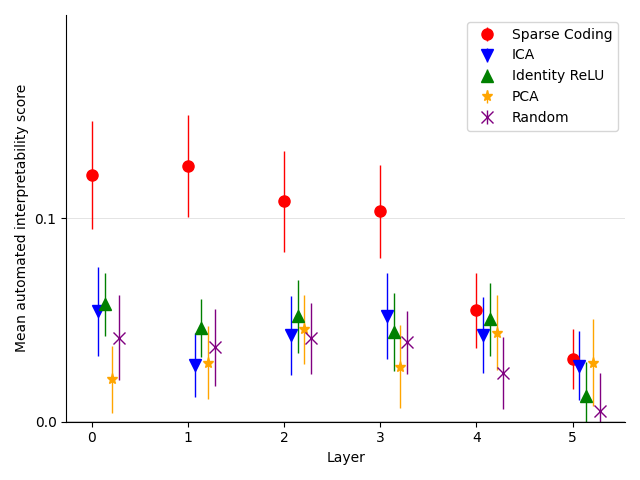
\includegraphics[width=0.8\textwidth]    {images/residual_random_means_and_cis_new.png}
    \caption{Random-only interpretability scores across each layer, a measure of how well the interpretation of the top activating cluster is able to explain the entire range of activations.}
    \label{fig:residual_random_activations}
\end{figure}

While the residual stream can usually be treated as a vector space with no privileged basis (a basis in which we would expect changes to be unusually meaningful, such as the standard basis after a non-linearity in an MLP), it has been noted that there is a tendency for transformers to store information in the residual stream basis\citep{dettmers2022llm}, which is believed to be caused by the Adam optimiser saving gradients with finite precision in the residual basis\citep{elhage2023privileged}. We do not find residual stream basis directions to be any more interpretable than random directions.


\subsection{Interpreting the MLP Sublayer}

Our approach of learning a feature dictionary and interpreting the resulting features can, in principle, be applied to any set of internal activations of a language model, not just the residual stream. Applying our approach to the MLP sublayer of a transformer resulted in mixed success. Our approach still finds many features that are more interpretable than the neurons. However, our architecture also learns many dead features, which never activate across the entire corpus. In some cases, there are so many dead features that the set of living features does not form an overcomplete basis. For example, in a dictionary with twice as many features as neurons, less than half might be active enough to perform automatic interpretability. The exceptions to this are the early layers, where a large fraction of them are active. 

For learning features in MLP layers, we find that we retain a larger number of features if we use a different matrix for the encoder and decoder, so that Equations \ref{eq:encoder} and \ref{eq:decoder} become

\begin{eqnarray}
\mathbf{c} &=& ReLU(M_e\mathbf{x}+\mathbf{b}) \label{eq:untied_encoder}\\
\mathbf{\hat x} &=& M_d^T \mathbf{c} \label{eq:untied_decoder}
\end{eqnarray}

\begin{figure}
    \label{fig:topk_mlp}
    \centering
    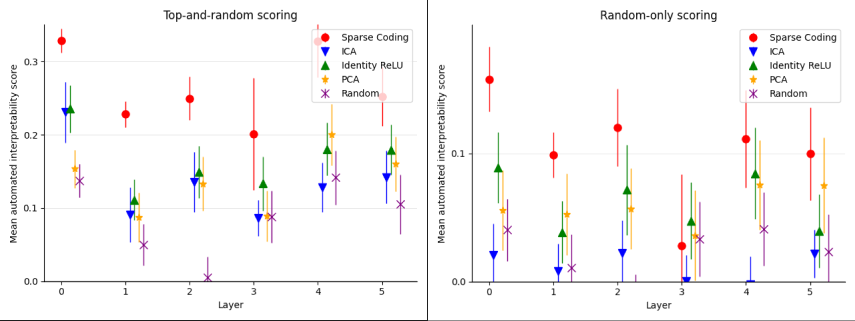
\includegraphics[width=.9\textwidth]{images/combomlp.png}
    \caption{Top-and-random and random-only interpretability scores for across each MLP layer, using an $\ell^1$ coefficient $\alpha=3.2e-4$ and dictionary size ratio $R=1$.}
\end{figure}


We are currently working on methods to overcome this and find truly overcomplete bases in the middle and later MLP layers.

\subsection{Interpretability Scores Correlate with Kurtosis and Skew of Activation}

It has been shown that the search for sparse, overcomplete dictionaries can be reformulated in terms of the search for directions that maximise the $\ell^4$-norm \citep{qu2019analysis}.

We offer a test of the utility of this by analysing the correlation between interpretability and a number of properties of learned directions. We find that there is a correlation of 0.19 and 0.24 between the degree of positive skew and kurtosis respectively that feature activations have and their top-and-random interpretability scores, as shown in Table \ref{tab:moment_correlation}.

\begin{table}[h]
    \centering
    \begin{tabular}{|c|c|}
        \hline
        \textbf{Moment} & \textbf{Correlation with top-random interpretability score} \\
        \hline
        Mean & -0.09\\
        \hline
        Variance & 0.02 \\
        \hline
        Skew & 0.20 \\
        \hline
        Kurtosis & 0.15 \\
        \hline
    \end{tabular}
    \caption{Correlation of interpretability score with feature moments across residual stream results, all layers, with dictionary size ratios $R \in \{0.5, 1, 2, 4, 8\}$.}
    \label{tab:moment_correlation}
\end{table}

This also accords with the intuitive explanation that the degree of interference due to other active features will be roughly normally distributed by the central limit theorem. If this is the case, then features will be notable for their heavy-tailedness.

This also explains why Independent Component Analysis (ICA), which maximises the non-Gaussianity of the found components, is the best performing of the alternatives that we considered.
